)\documentclass{article}[11pt]
\usepackage[portrait, margin=1in]{geometry}
\usepackage{graphicx} 
\graphicspath{{/Users/danpost/housing_project/output/prospectus/graphics}}
\usepackage{amsmath}
\usepackage{hyperref}
\usepackage{booktabs}
\usepackage{array}
\usepackage[authordate, backend=bibtex, natbib]{biblatex-chicago}
\addbibresource{prospectus_bib.bib}

\begin{document}

\title{Housing Policy, Access to Capital, and the Construction of Political Coalitions} 
\author{Daniel Posthumus}

\maketitle

\section{Introduction}
Why, as labor productivity, output, and aggregate demand have all increased, has the United States gotten worse at building things? This is a question whose answer we understand fairly well; burdensome regulation has made it more difficult to build. This is the core argument of the ``abundance agenda" (also referred to as ``supply-side progressivism"), which liberal commentators (most prominently Ezra Klein and Derek Thompson) have centered in their arguments over why Democrats lost the election in 2024 and how liberalism can redeem itself.\footnote{Although the idea of supply side progressivism preceded the 2024 election, and went hand-in-hand with the post-COVID development of Bidenomics. The agenda has two leading focuses: energy and housing. In this paper, I focus on the latter; I conceive of housing and energy policy as wholly distinct and the result of distinct political processes (energy being largely determined at the state/federal level, while housing policy is largely determined at the local level). For an introduction to the way the abundance agenda addresses energy, see \citep{cheap2022energy}. While the abundance agenda motivates the urgency of the puzzle I identify, I don't center it in this paper.} \citep{klein2021economic} \citep{kleinthompson}

With respect to housing, the abundance agenda highlights a basic misallocation problem: it is very hard to move to the most productive places in the United States of America. It's hard because housing is too expensive there: construction and supply in these places has not kept up with demand because of burdensome regulation has choked off supply. \citep{glaeser2005} \citep{glaeser2005empirical} The economics of this are well-established; scholars have demonstrated that housing prices are higher because of land-use regulation, and they have demonstrated this has led to a misallocation of labor which has devastating effects on aggregate output. \citep{hsieh2019housing} In this framing, politics, not economics, has prevented the ``invisible hand" of the market from operating. In this version, \textit{housing markets are out of equilibrium}. Klein and Thompson have a simple solution: remove the bottleneck of politics, and markets will achieve equilibria and prices will come down.

This argument is well-founded, although I think its literature neglects two areas: politics and credit access.\footnote{Again, my focus here is on the academic literature, not the work in popular media by bloggers/writers like Matt Yglesias, Noah Smith, Klein, and Thompson. However, many of the flaws in the literature are reflected in the work of this bloggers. The literature's lack of understanding of politics in developing regulations for example, can be reflected back as these bloggers' lack of awareness. To pick an easy example, a recent \href{https://www.slowboring.com/p/new-york-city-can-do-better-than}{article} by Yglesias' media company \textit{Slow Boring} touts a New York City mayoral candidate Zellnor Myrie for his pro-housing policies. \citep{zellnor} Myrie is, according to \href{https://poll.qu.edu/images/polling/nyc/nyc03052025_nytv24.pdf}{Quinnipac}, polling at 1\%. This gap--between Myrie's popularity among `thinking liberals' and his popularity with voters--is not seriously addressed in the piece and is part of a broader overlooking of popular politics among Abundance thinkers.} First, housing policies are endogenous; they are, by definition, the result of political processes which are determined by constituents -- the composition of which is dependent on who can afford the housing in a community. I propose new ways to incorporate politics into structural models of housing and address housing policies' endogeneity issues. Second, the literature does not adequately incorporate access to credit into models; in particular, we don't understand how interventions in credit markets affect housing markets.

There are many ways to approach these challenges, and I am not close to formalizing a model and presenting results. What I do in this paper is first prove there is a puzzle that needs to be answered: \textbf{we don't have a complete model of housing market equilibrium or disequilibrium that effectively incorporates 1) politics and 2) credit access}. This puzzle matters: housing policy is deeply broken in America, but to fix it people need to understand how to structure capital access, and the political processes which produce and result from the very housing regime that economists have thoroughly demonstrated is economically broken. 

In the second half of this paper, I explore some specific ways I can operationalize and understand this broad theme. One little-understood question that politicians and policymakers want an answer to are the effects of the Community Reinvestment Act (CRA). I briefly discuss previous work on the CRA, before proposing new research on its effects on housing markets through expansions (or contractions) in credit access. Another proposal is to harness the richness of zoning commission hearing data through the most novel Natural Language Processing (NLP) methods to develop rich data on the political \textit{process} of regulation-making, something we simply don't have good data on but would be a good way of overcoming the endogeneity of housing policy. Finally, I conclude with the broad brush strokes of a historical project. We don't know have a good idea of what housing markets looked like before zoning; I propose an expansion on previous work using historical newspapers to develop a real estate listing-level dataset for the pre-zoning era. These ideas can be disparate (and threateningly unwieldy) at times and not all provide solutions to the puzzle I lay out; however, I believe that the ultimate goal of these ideas is to produce separate pieces of empirical evidence which can then be synthesized into a theoretical expansion in how we thinking about housing, the ideas of which I conclude this paper.

\section{Literature Review}

The research puzzle I identify lies at the intersection of different literatures, each of which is vast and unwieldy to summarize. I focus on the broad strokes of 3 literatures. First, I establish that a large literature finds that exclusive and constrictive land use regulation exists in the United States and that this regime has harsh, negative economic effects through raising prices and 2nd- or 3rd-order effects such as labor misallocation and lower construction productivity. Some papers have addressed regulation's endogeneity, although this remains an unsolved challenge. Second, I demonstrate that some scholars have focused on the role of credit access in shaping housing markets. This literature is distinct and unconnected to empirical work on regulation and structural housing models, even though the very notion of credit access is deeply embedded in housing markets. I argue it needs to be integrated into how we think about housing. Finally, some scholars have previously tried to build structural models of housing markets which explain why land use regulation exists. Empirical findings have largely not corroborated the theoretical stories of these models. I focus on how these models fail to incorporate politics and credit access.
		
	\subsection{Land Use Regulation}
In the early-mid 2000s, an influential series of articles appeared first establishing the existence of exclusionary zoning restrictions and demonstrating these restrictions were leading to increased housing prices. Although previous work was aware of this phenomenon and its effects, the mid 2000s wave of papers was critical in systematizing our understanding of regulation and its effects. Fischel (2004) provides a thorough economic historic review for \textit{why} exclusionary zoning policies exist. \citep{fischel2004economic} Fischel was prominent for developing a theory that homeowners became \textit{homevoters}, i.e., they would vote for their homes in local elections and at public hearings. Homeowners have a significant financial asset that can increase in value through the achievement of certain policies, so they will push hard for those policies. Fischel's theory is also that homeowners tend to be commuters; hence zoning's initial coinciding with the expansion of streetcar suburbs in the 1910s and 20s and its later expansion under suburbanization and urban renewal in the 1950s and 60s.\footnote{Fischel's approach may seem slightly dated to the reader in 2025; he argued that homeowners were worried about their homes \textit{losing} value, and that zoning was protection against that possibility through increases in density. Today, one might take for granted homes in high-productive areas with restrictive land regulations are perpetually gaining in value, such that when one buys a home one expects not just a steady investment, but significant appreciation over time. This distinction is not central to what I see as Fischel's main contribution, which is explaining the emergence of these regulations between 60-100 years ago, but I think it merits mention.} 

The basic fact of constrictive zoning regulations established, I turn to its effects. Pre-2005, Quigley and Rosenthal document a breadth of papers showing an association, though not causal relationship, between land use regulation and housing prices. \citep{quigley2005effects} Glaeser et al. built on this work to more thoroughly solve a puzzling phenomenon: the cost of building a house stagnated from 1970 to 2005, while housing prices increased astronomically. \citep{glaeser2005empirical} Their argument was that the literature had previously focused on demand-side explanations, while the truth lie on the supply side, which was constrained by restrictive zoning regulations. While Glaeser et al.'s empirics are largely descriptive, they spawned analysis of further effects of zoning regulation beyond the 1st-order price effects.\footnote{Glaeser et al.'s empirics focus on disproving alternative explanations for the divergence of housing prices and construction costs. They show that only about a quarter of this gap could be explained by increases in housing quality. Next, they show that high demand (measured by the ratio of price to construction costs) in the 1970s drove new construction in the following decade, whereas that basic relationship was reversed as soon as the 1990s. \textit{High prices no longer led to new construction}, suggesting the reason for those high prices is not high demand, but low supply which can't easily be expanded. They formalize some of these ideas into a model which I briefly discuss below.} 

Housing prices have tremendous 2nd-order and 3rd-order effects: if housing prices increase in a given area, fewer people can afford to live there. This may lead to spatial misallocation of workers if the most productive firms are located in places with stricter regulations and higher prices (prominently San Francisco, for example). Hsieh and Moretti find that if San Francisco, New York City, and San Jose reduced land use regulations to the level of the median city, their growth rate of aggregate output would be 36.3 percent higher -- resulting in a stunning 3.7\% increase in US GDP in 2009.\footnote{This finding and its magnitude serve as a key motivator for the abundance agenda, although notable critiques of the abundance agenda's focus on increasing the aggregate output of these high-productive metros wonder why the movement wouldn't focus on increasing productivity in less-productive areas. \citep{abundanceambiguity}}\footnote{Also, more restrictive zoning policies have also been associated with a great share of residents commuting and working in another community in California. \citep{durst2021land}}  \citep{hsieh2019housing} Another proposed effect of regulation is a weakening of construction productivity, specifically the growing gap between manufacturing traded good productivity and construction productivity in the United States. D'Amico et al. (2024) demonstrate that constrictive regulation has resulted in smaller construction firms and smaller construction projects, which accounts for a very large share of the gap between manufacturing and construction productivity. \citep{d2024has} \footnote{There are other exciting advances in this literature. Bartik et al. use Large Language Models (LLMS) to interpret statutes and create advanced non-survey-based data on zoning laws. \citep{bartik2024costs} Gabriel and Kung find regulations manifest in extreme development approval times, reducing housing production and productivity through a construction-level dataset. \citep{gabriel2024development} Glaeser and Ward find that restrictive regulations cause less construction and higher prices, unless you control contemporary neighborhood characteristics such as demographics and density. \citep{glaeser2009causes} Of course, if we accept that regulations cause lower density, then its lack of significance upon controlling for density in no way means it doesn't have an upward effect on prices.}

	\subsection{Credit Access and Housing Markets}
	


	\subsection{Regulation Emergence and Structural Modeling}
Scholars have been far less successful in demonstrating why these regulations emerge than they have been in conclusively proving their effects. In short, \textit{there's little empirical evidence that a larger share of homeowners in a given population leads to greater support for exclusionary zoning restrictions}, i.e., the homevoter hypothesis. In this section, I review the implications and design of some prominent models and explain how they fail to treat 

I don't discuss every structural modeling of housing; I focus here on Several scholars have built structural models, attempting to formalize Fischel's and others' theories about why zoning policies have taken hold. Glaeser et al. built a model to explain the choices faced by homeowners and landlords, one key insight of which is that the development level of a neighborhood which maximizes \textit{current residents'} welfare is not socially optimal, in large part because current homeowners' utility rises with the value of their homes, and they have no internalization of the harmful effects of these rising home prices (and, accordingly, rents) on those who want to live in the town but can't afford to. \citep{glaeser2005} They conclude with some ideas about why exclusionary restrictions have taken hold.\footnote{Their first proposition relates to the composition of local political organizing: conditional on homeowners associations (HOAs) and landlords \textit{both} lobbying for more restrictive zoning conditions, landlords will expend cash while HOAs will expend time. This is not directly related to my research but interesting to note.} One explanation is that ``judicial tastes" and political decision-makers' preferences for development have shifted. Another is that home-ownership is more common. A final possible explanation is that low density communities are normal goods; as incomes rise, people want to live in a low density community. 

Other structural models exist; Ortalo-Magné and Prat (2014) build one in which the central tradeoff for households is between short-term rents (which they pay to themselves if they own their house or absentee landlords if they're renting the property) or end-of-period consumption. \citep{ortalo2014political} If the housing supply goes up, rents go down but housing wealth, consumed at the end of an individual's life, goes down -- and vice-versa. Much like Glaeser et al., their model is rich and convincing in modeling households' incentives vis-a-vis policy. However, it overlooks political constraints and neglects households' access to capital. 

	\subsection{The Puzzle}



	\subsection{Data}
The empirical analyses I discuss above were largely limited by the lack of a comprehensive dataset on zoning restrictions and housing policy in general; since the publication of his 2005 paper with co-authors, Gyourko has compiled two waves of a nation-wide survey on local regulatory environments, one in 2007 and the other in 2021. \citep{gyourko2008new} \citep{gyourko2021local} \footnote{To summarize, they sought data on 1) general characteristics of the regulatory process, 2) specifics of the local residential land use regulation, 3) outcomes of the regulatory process, 4) state-level analyses of land use policy actions, and 5) measures related to environmental and open space-related ballot initiatives (the latter two categories of variables weren't directly part of the survey but were supplemented by the authors' own analysis.} Another prominent survey, the Terner California Residential Land Use Survey, focuses on California--although it has the drawback of only having one wave of data, from 2017-2018. \citep{mawhorter2018terner} In general, data has lagged behind formal modeling as it relates to housing supply exclusionary zoning -- \textit{particularly along the dimension of time}. \citep{gyourko2015regulation} Nonetheless, extensive progress has been made in data for urban and regional economics the last 10 years. \citep{newdata} With regard to historical data, much of this work has been made by digitizing paper maps (to obtain census tract- or neighborhood-level boundaries used to geographically categorize households, that we could pull from historical Census records, the complete microdata of which is released 72 years after it was fielded). These historical maps and linked census data have allowed researchers to track historical neighborhood formation and segregation within cities. Work is currently underway to use NLP methods to create a true nation-wide dataset on local zoning ordinances, which does \textit{not} rely on survey methods like Gyourko et al. does. \citep{bartik2024costs} 

\section{Operationalizing The Puzzle}

	\subsection{Community Reinvestment Act (CRA) of 1977}
Created in an attempt to remedy redlining, the Community Reinvestment Act (CRA) of 1977 creates a framework of regulations for how federal banking regulatory agencies ensure that banking institutions meet the credit needs of low- and moderate-income (LMI) neighborhoods.\footnote{Redlining refers to the practice wherein lenders and insurance providers would shade neighborhoods `red' on maps that were predominantly Black which they would not service and would discriminate against. In the 1930s and 1940s there was no legal protection against this practice. For an effective introduction into the practice of redlining and its embeddedness in credit markets, see \cite{hillier2003redlining}.} \footnote{The federal banking regulatory agencies are specifically the Federal Reserve's Board of Governors, the Federal Deposit Insurance Corporation (FDIC), and the Office of the Comptroller of the Currency (OCC).} The CRA has undergone several waves of formal regulatory changes and concerns about its effectiveness have hampered its enforcement. \footnote{Regulatory changes came in three  primary waves: 1) in 1989, agencies were required to publicly disclose how well banks were meeting the requirements laid out in the CRA; 2) in 1995, the CRA's bank tests were customized for different types of banks; and 3) in 2005, bank size definitions were made in real terms, indexed by the Consumer Price Index (CPI).} The details of the CRA are technical and not in the scope of this prospectus (I lay out the features of its design relative to my research below); for a review of its contents, Getter from the Congressional Research Service (CRS) has prepared a very effective overview. \citep{getter2015effectiveness} Here I focus on demonstrating why the CRA is important and the puzzle as to its effectiveness, in particular its relationship to the housing market literature I've laid out above.

There are several challenges to determining CRA effectiveness. \citep{getter2015effectiveness} CRA examinations leave significant room for examiner subjectivity and discretion; as of 2015, there were no specific definitions of criteria or quantitative quotas associated with examination ratings. There's also little variation in bank success in passing the examine; from 2006 to 2014, in no single year were more than 3.5\% of banks rated noncompliant or needs to improve. In general, CRA-qualified investments also proved to be  profitable, making it difficult to parse the profit motive for a bank's investment compared to CRA-induced incentives. As a result of these challenges, there is no consensus over the effects of the CRA -- particularly over its effects on the housing loans, discrimination in which it was originally designed to combat.

		\subsubsection{The Puzzle}
Research on the CRA and housing is extremely limited. One prominent studied, authored by Saadi, demonstrates that enhanced CRA enforcement -- beginning in 1998 -- increased mortgaged lending to CRA-eligible neighborhoods, fueling home pricing, and ultimately resulting in a worse housing bust in these neighborhoods post-2008. \citep{saadi2020role} I want to focus on Saadi's identification strategy, which exploits the CRA's institutional features. The first is that the policy change in 1998 was exogenous to local housing conditions in any given community. Second, is that CRA eligibility is relative to Metropolitan Statistical Area (MSA) median household income, meaning there are two variables in determining CRA eligibility: census tract median household income and MSA median household income. This means that we can find variation in CRA eligibility even across tracts with similar median household incomes, because of variation in MSA median household income.\footnote{Specifically, the CRA requires a census tract's median household income fall below 80\% of the MSA median household income.} This is fine, but Saadi makes a sweeping assumption; \textit{because we can control for tract-level income and maintain variation in CSA variation, there won't be omitted variable bias.} \textbf{Saadi is making the same mistake Glaeser et al. criticized the literature on housing of doing back in 2005}: focusing on demand-side variables. \citep{glaeser2005empirical} The third feature Saadi highlights is that not all institutions are subject to the CRA. Saadi then demonstrates that 1) the 1998 change in CRA enforcement increased loans to CRA-eligible tracts (along the \textit{extensive} margin, i.e., this increase was driven by the number not size of loans); 2) credit availability has a causal link to housing prices; and 3) the CRA raised housing prices through credit availability.

There are two critiques of Saadi's work and why it doesn't solve the puzzle I've laid out of fitting credit access into models of housing. The first, pointed out by Brevoort, is that Saadi's facts are plain wrong. \citep{brevoort2024reexamining} Saadi relied on a secondary source to ascertain that the Clinton-era change in CRA enforcement took place in 1998, whereas directly consulting the \textit{Federal Register} reveals the enforcement change went into action on January 1, 1996, 2.5 years before 1998. Instead, Brevoort argues, what happened in 1998 was Russia defaulting on its debt, leading to a `flight to quality'. Subprime lenders, primarily non-banks, were bought by banks, making LMI lending appear on banking balance sheets starting in late-1998, lending that was previously on the non-banking sector's balance sheet. Replicating Saadi's research design, using 1996 as the point of exogenous change in CRA enforcement rather than 1998 results in finding no effects of CRA enforcement on credit access and thus the subprime crisis.

The second critique deals with Saadi's complete disregard for politics. It may seem strange for a paper whose outcome of interest is housing prices to not mention zoning and regulations \textit{once} after I exhaustively demonstrated the empirical evidence on restrictive regulations' effects on housing prices. This isn't that surprising, however, because the housing models that attempt to explain housing markets and zoning regulations, largely ignore access to credit. Each story feels incomplete, and is without the other.

		\subsubsection{Ideas for Research Design}
Saadi's empirical strategy relies on a single faulty fact which, when corrected, invalidates his approach; this doesn't, however, mean we can't try to understand changes in credit access and their effects on housing markets. In this section, I describe some ways to analyze the effect of the CRA on credit access in housing markets. CRA enforcement is complex; I don't claim to have a rock-solid identification strategy, which will require deeper immersion into the institution features of CRA enforcement, credit markets, and banking regulation.



		\subsubsection{Reduced Form Evidence}



	\subsection{Other Ideas For Operationalization}
		
		\subsubsection{Zoning Commissions}
A natural place to start if we're interested in how housing markets are designed through political processes are the processes themselves, which are very poorly understood. \citep{gyourko2015regulation} Recent advances in NLP methods have allowed researchers to comb through documents whose sheer size made them previously impossible to parse in order to build datasets of zoning regulations. \citep{bartik2024costs} Most decisions--such as variances, special use permits, and cities' comprehensive plans--are made by bodies such as Boards of Zoning Adjustment or Zoning Appeals (BZAs) or Planning and Zoning (P\&Z) commissions. \citep{anderson2008study} While work has been done on the composition of these bodies (focusing on whether they are composed of the ``ordinary citizen"), little to no work has been done on developing exhaustive datasets on these bodies' \textit{actions}.

Intuitively, this dearth of work isn't surprising if one tries to read, much less understand, the minutes of such hearings -- even if the sheer quantity of information is very rich. The \href{https://sfplanning.org/cpc-hearing-archives}{SF Planning Commission}, for example, has agendas and minutes dating back to 1998 \textit{for weekly meetings}. A typical item in the minutes appears in the appendix of this paper as Figure \ref{sf_zoning_example_1}. Another richer, more interesting datapoint would be that featured in Figure \ref{sf_zoning_example_2}, since this is a resolution that was actively voted on, not just put up for continuance.\footnote{The example was taken from the Thursday, December 12, 2024 Meeting. That meeting's minutes can be found \href{https://citypln-m-extnl.sfgov.org/Commissions/Agenda_or_Minutes/20241212_cpc_min.pdf}{here}.}



There are also challenges in parsing this data. How do we consistently operationalize the description of the project?\footnote{The description of this project is: ``Request for \textbf{Discretionary Review} of Planning Application No. 2024-000521PRJ for the demolition of a one-story over basement single family house and new construction of a three-story over basement, two-unit building....} General public comments, which don't adhere to the same standardized formatting as items put up for the commission's consideration, would also be much harder to parse using NLP methods.

Then, taken together, we can answer all sorts of descriptive questions. We can create a project-level dataset tracking projects over time, a commission member-level dataset tracking members' votes over time, or a location-based dataset. San Francisco, in the 2020 Census, had 244 census tracts \textit{within} city limits. Tract-level data on housing construction, income, demographics, etc. are straightforward to find. Furthermore, CRA eligibility is determined at the tract level. The creation of this dataset would be novel; it would require work from NLP methods, but those methods are demonstrated to have borne tremendous fruit in this sub-literature already. Detailed data on the \textit{process} of zoning regulations, not just outcomes, would unlock--most importantly--the dynamic nature of regulation-making, a key challenge to overcoming the endogeneity of housing policy as either treatment or outcome.

		\subsubsection{Constructing History}
Fischel posits that New York City was among the first cities to implement city-wide zoning, in 1916. \citep{fischel2004economic} Pre-zoning city formation would then not be burdened by the problem of endogenous housing policy; however, pre-1975 housing data is scarce. In June 2024, Lyons et al. published the first comprehensive city-level sales/rent indices, covering 1890 and 2006. \citep{lyons2024price} Their dataset relies on digitized newspaper archives of major cities.\footnote{The full list of their newspaper sources can be found \href{https://www.philadelphiafed.org/surveys-and-data/data-sources}{here}. The home of their data can be found \href{https://www.philadelphiafed.org/surveys-and-data/regional-economic-analysis/historical-housing-prices}{here}.} This data is rich--and a vast improvement over the spliced historical index used before--and provides a promising start for the construction of comprehensive historical housing dataset; however, it's limited. 

I'm interested in expanding the depth of the project, focusing on San Francisco. Owners of SF-based newspapers during the Gilded Age were deeply invested in real estate; they sought to establish SF as a center of imperialism over the Pacific Ocean to increase industrial activity in the city and thus increase the value of real estate. \citep{brechin2006imperial} Lyons et al. construct their housing index from listings in only one SF newspaper -- the \textit{Chronicle}. The de Young brothers owned the Chronicle; as Berchin demonstrated, M. H. de Young was deeply invested in real estate. For example, de Young used his political influence pushed to host the International Exposition of 1894 in Golden Gate Park: after all, he owned 31 blocks south of the park. De Young did not shy away from directly meddling in his paper's content; clearly, relying on the real estate listings in his paper as representative of housing conditions in \textit{all} of San Francisco would not be entirely accurate (although it would likely suffice for the purpose of Lyons et al.'s work).

In the second half of the 19th century, there was furious competition between the De Youngs and two other titans -- John D. Spreckels (owner of the \textit{San Francisco Call} and William Randolph Hearst (owner of the \textit{San Francisco Examiner}). Each owned significant real estate in the city and aggressively used their newspapers to advance their commercial interests. While perhaps not directly related to the puzzle I laid out in this paper, I think building a detailed dataset of the real estate listings contained in these newspapers (focusing on these three, the most significant for their owners' commercial interests) would be instrumental for understanding what the politics of city formation were in the pre-zoning era.

With this advanced dataset, we could better understand the effect of the first electric railways (the first streetcar in San Francisco opened in 1892) on patterns of construction and real estate prices. The Outside Lands of San Francisco (referring to the Richmond and Sunset Districts) were only developed around 1870, when the city developed Golden Gate Park. This provides a unique opportunity; we can model the physical geographic characteristics of property in these Outside Lands, before they were thoroughly developed, and predict patterns of housing development. These generated patterns of housing development would be compared to the actual housing development, per the listing data I developed from the newspapers described above. We can imagine this approach including more and more fundamental variables, down to trying to understand who owned what property in the Outside Lands (think the 31 blocks south of Golden Gate Park that De Young owned). Such an approach would be part of a larger push in the literature for an ecological approach to modeling political economic outcomes. \citep{haber2021ecological}

\section{Conclusion}

	\subsection{Expanding Theoretical Frameworks for Housing Political Economy}
	
\clearpage

\section{Appendix}

	\subsection{Operationalization of SF Zoning Commission's Continuance Resolution Example}
	
As another example how NLP methods would possible parse the Zoning Commission's meeting minutes (see Figure \ref{sf_zoning_example_1}, I extract the following variables:
\begin{itemize}
	\item \textbf{Date of meeting}: December 12, 2024
	\item \textbf{Type of Action}: Continuance
	\item \textbf{Request made}: Conditional Use Authorization
	\item \textbf{Exact location of project}: 411 Clipper Street, San Francisco
	\item \textbf{Type of zoning district}: RH-2 (Residential-House, Two Family)
	\item \textbf{Height and bulk district}: 40-X
	\item \textbf{Exemption from California Environment Environmental Quality (CEQA)}: Yes
	\item \textbf{Speakers}: 0
	\item \textbf{Action}: Continuance (until January 16, 2025)
	\item \textbf{Ayes - Nayes}: 7-0 
\end{itemize}

	\subsection{Figures}
	
		\begin{figure}[h]
		\centering
			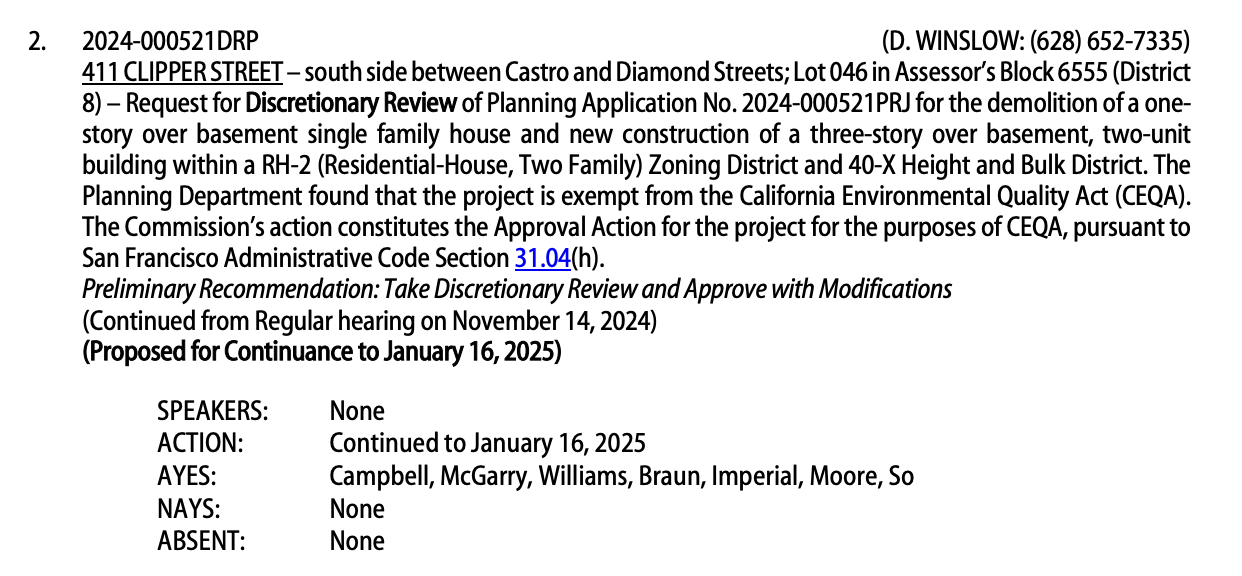
\includegraphics[width=0.8\textwidth]{sf_zoning_example_1.png}
			\caption{Example of Information Contained in San Francisco Planning Commission Meeting Minutes}
			\label{sf_zoning_example_1}
		\end{figure}
	
\clearpage
\printbibliography

\end{document}